\definecolor{singleShotColor}{RGB}{196,106,28}
\definecolor{pipelineColor}{RGB}{44,138,100}
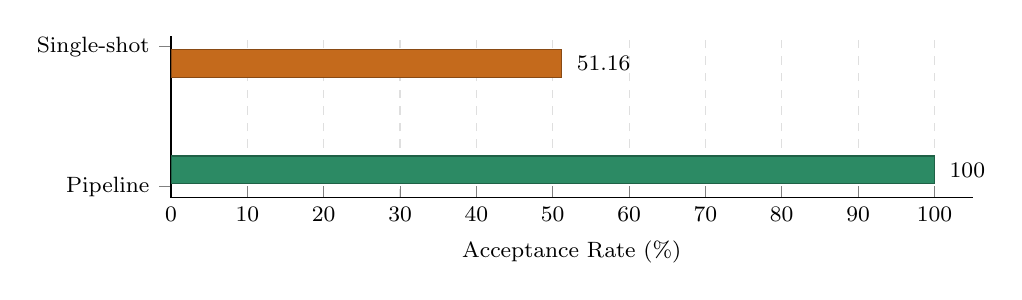
\begin{tikzpicture}
\begin{axis}[
    xbar,
    width=0.97\columnwidth,
    height=0.30\columnwidth,
    xmin=0,
    xmax=105,
    xlabel={Acceptance Rate (\%)},
    symbolic y coords={Pipeline,Single-shot},
    ytick={Single-shot,Pipeline},
    yticklabels={Single-shot,Pipeline},
    enlarge y limits={abs=4pt},
    axis lines*=left,
    xmajorgrids=true,
    grid style={dashed,gray!25},
    tick label style={font=\footnotesize},
    label style={font=\footnotesize},
    nodes near coords,
    every node near coord/.append style={font=\footnotesize, text=black, anchor=west, xshift=2pt},
]
\addplot+[fill=singleShotColor, draw=singleShotColor!70!black] coordinates {
    (51.16,Single-shot)
};
\addplot+[fill=pipelineColor, draw=pipelineColor!70!black] coordinates {
    (100.00,Pipeline)
};
\end{axis}
\end{tikzpicture}
